\chapter{Résultats et Discussion}     % numéroté chap4
\thispagestyle{fancy}
Après avoir réalisé une conception qui répondait bien aux besoins de l’application, nous entamons la partie amélioration de l’application IZIWAY CAMEROUN, en exposant les différents outils de langages de développement utilisés lors de la réalisation et l’implémentation de la base de données ainsi qu’un aperçu sur les interfaces de notre application.

\section{Outils, langage et méthodes d’implémentations.}

\subsection{Outils d'implémentation.}

Le développement d’un tel système nécessite l’utilisation de quelques outils. Dans ce qui suit nous citons les outils qui ont été utilisés.

\textbf{SQL Server  :} 

Microsoft SQL Server est un système de gestion de base de données (SGBD) en langage SQL incorporant entre autres un SGBDR (SGBD relationnel ») développé et commercialisé par la société Microsoft. Il fonctionne sous les OS Windows et Linux (depuis mars 2016), mais il est possible de le lancer sur Mac OS via Docker, car il en existe une version en téléchargement sur le site de Microsoft.

\textbf{Visual Studio   :} 

Visual Studio est un ensemble complet d'outils de développement permettant de générer des applications web ASP.NET, des services web XML, des applications bureautiques et des applications mobiles. Visual Basic, Visual C++, Visual C\# utilisent tous le même environnement de développement intégré (IDE), qui leur permet de partager des outils et facilite la création de solutions faisant appel à plusieurs langages.

\subsection{Langages de programmation utilisés.}

\textbf{Langage SQL   :} 

SQL (Structured Query Language) en français « Langage d’interrogation Structuré », est un langage d’interrogation de base de données très populaire. Il constitue aujourd’hui une norme implémentée par de nombreux SGBDs (Systèmes de Gestion de Bases de Données), comprenez : des serveurs de bases de données. L’accès aux BDD (bases de données) se fait de façon standard à l’aide de requêtes du langage SQL. Il existe un outil d’administration, MySQL Management, qui nous offre une interface pour manipuler les tables. La connaissance de quelques requêtes permet de répondre à la majorité des besoins de programmation.

\textbf{C\#   :} 

C\# (prononcé voir dièse, comme la note de musique , mais écrit avec le signe du nombre) est un langage de programmation multi-paradigme à usage général, englobant des disciplines de programmation à typage fort, à portée lexicale, impérative, déclarative, fonctionnelle, générique, orientée objet (basée sur la classe) et orientée composant. Il a été développé vers 2000 par Microsoft dans le cadre de son initiative .NET et a ensuite été approuvé comme norme internationale par Ecma (ECMA-334) en 2002 et ISO (ISO/IEC 23270) en 2003. Mono est le nom du projet libre et open-source visant à développer un compilateur et un runtime pour le langage. C\# est l'un des langages de programmation conçus pour l'infrastructure linguistique commune (CLI).

\textbf{Flutter   :} 

Flutter est un kit de développement de logiciels d'interface utilisateur à source ouverte créé par Google. Il est utilisé pour développer des applications pour Android, iOS, Linux, Mac, Windows, Google Fuchsia et le web à partir d'une seule base de code. La première version de Flutter était connue sous le nom de code "Sky" et fonctionnait sur le système d'exploitation Android. Elle a été dévoilée lors du sommet des développeurs Dart de 2015, avec l'intention déclarée de pouvoir effectuer un rendu cohérent à 120 images par seconde. Lors du discours d'ouverture des Google Developer Days à Shanghai, Google a annoncé la sortie de Flutter Release Preview 2 qui est la dernière grande version avant Flutter 1.0. Le 4 décembre 2018, Flutter 1.0 a été publié lors de l'événement Flutter Live, ce qui représente la première version "stable" du Framework. Le 11 décembre 2019, Flutter 1.12 a été publié lors de l'événement Flutter Interactive.

\section{Présentation de la solution réalisée}

\subsection{Architecture MVC de l'application.}

Le patron de conception modèle-vue-contrôleur (en abrégé MVC, en anglais model-view-controller), tout comme les patrons modèle-vue-présentation ou présentation, abstraction, contrôle, est un modèle destiné à répondre aux besoins des applications interactives en séparant les problématiques liées aux différents composants au sein de leur architecture respective. 

Ce paradigme regroupe les fonctions nécessaires en trois catégories :

\begin{enumerate}
	\item  \textbf{Un modèle :}
	Le modèle représente le cœur (algorithmique) de l’application : traitements des données, interactions avec la base de données, etc. Il décrit les données manipulées par l’application. Il regroupe la gestion de ces données et est responsable de leur intégrité. La base de données sera l’un de ses composants. Le modèle comporte des méthodes standards pour mettre à jour ces données (insertion, suppression, changement de valeur). Il offre aussi des méthodes pour récupérer ces données. Les résultats renvoyés par le modèle ne s’occupent pas de la présentation. Le modèle ne contient aucun lien direct vers le contrôleur ou la vue. Sa communication avec la vue s’effectue au travers du patron observateur. Le modèle peut autoriser plusieurs vues partielles des données. Si par exemple le programme manipule une base de données pour les emplois du temps, le modèle peut avoir des méthodes pour avoir tous les cours d’une salle, tous les cours d’une personne ou tous les cours d’un groupe de TD.
	\item  \textbf{Une vue :}
	Ce avec quoi l’utilisateur interagit se nomme précisément la vue. Sa première tâche est de présenter les résultats renvoyés par le modèle. Sa seconde tâche est de recevoir toute action de l’utilisateur (hover, clic de souris, sélection d’un bouton radio, cochage d’une case, entrée de texte, de mouvements, de voix, etc.). Ces différents événements sont envoyés au contrôleur. La vue n’effectue pas de traitement, elle se contente d’afficher les résultats des traitements effectués par le modèle et d’interagir avec l’utilisateur. 
	
Plusieurs vues peuvent afficher des informations partielles ou non d’un même modèle. Par exemple si une application de conversion de base a un entier comme unique donnée, ce même entier peut être affiché de multiples façons (en texte dans différentes bases, bit par bit avec des boutons à cocher, avec des curseurs). La vue peut aussi offrir à l’utilisateur la possibilité de changer de vue. 

	\item  \textbf{Un Controller :}
	Le contrôleur prend en charge la gestion des événements de synchronisation pour mettre à jour la vue ou le modèle et les synchroniser. Il reçoit tous les événements de la vue et enclenche les actions à effectuer. Si une action nécessite un changement des données, le contrôleur demande la modification des données au modèle afin que les données affichées se mettent à jour. D’après le patron de conception observateur/observable, la vue est un « observateur » du modèle qui est lui « observable ». Certains événements de l’utilisateur ne concernent pas les données mais la vue. Dans ce cas, le contrôleur demande à la vue de se modifier. Le contrôleur n’effectue aucun traitement, ne modifie aucune donnée. Il analyse la requête du client et se contente d’appeler le modèle adéquat et de renvoyer la vue correspondant à la demande. 
\end{enumerate}

Par exemple, dans le cas d’une base de données gérant les emplois du temps des professeurs d’une école, une action de l’utilisateur peut être l’entrée (saisie) d’un nouveau cours. Le contrôleur ajoute ce cours au modèle et demande sa prise en compte par la vue. Une action de l’utilisateur peut aussi être de sélectionner une nouvelle personne pour visualiser tous ses cours. Ceci ne modifie pas la base des cours mais nécessite simplement que la vue s’adapte et offre à l’utilisateur une vision des cours de cette personne. Quand un même objet contrôleur reçoit les événements de tous les composants, il lui faut déterminer l’origine de chaque événement. Ce tri des événements peut s’avérer fastidieux et peut conduire à un code peu élégant (un énorme switch). C’est pourquoi le contrôleur est souvent scindé en plusieurs parties dont chacune reçoit les événements d’une partie des composants. 

\begin{figure}[H]
	\centering
	\includegraphics[width=14cm]{MVC.png}
	\caption{Architecture MVC de l'application.}
	\label{fig:sp0}
\end{figure}

\subsection{Avantage du MVC.}

Un avantage apporté par ce modèle est la clarté de l’architecture qu’il impose. Cela simplifie la tâche du développeur lors de la maintenance ou d’une amélioration sur le projet. En effet, la modification des traitements ne change en rien la vue. Par exemple on peut passer d’une base de données de type SQL à XML en changeant simplement les traitements d’interaction avec la base, et les vues ne s’en trouvent pas affectées. Le MVC montre ses limites dans le cadre des applications utilisant les technologies du web, bâties à partir de serveurs d’applications. Des couches supplémentaires sont alors introduites ainsi que les mécanismes d’inversion de contrôle et d’injection de dépendance. 

\subsection{Page du tableau de bord.}

Le tableau de bord présente de manière globale toutes les informations de l’application, sous forme de graphes et chiffres statistique. On présente le nombre d’informations enregistrées, ensuite l’alerte, qui est l’avancement automatique, on présente les commandes.

\begin{figure}[H]
	\centering
	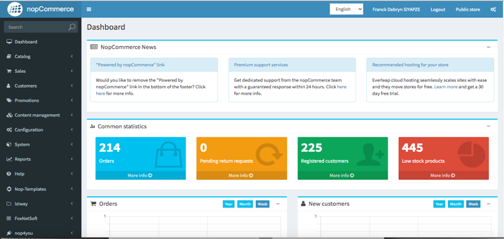
\includegraphics[width=16cm]{tableau_bord.png}
	\caption{Page du tableau de bord.}
	\label{fig:sp0}
\end{figure}

\subsection{Page de gestion des sliders.}

Dans cette page on présente les informations concernant les sliders. Le premier bloc représente l’ajout des sliders et le deuxième bloc la liste des sliders déjà implémentés.

\begin{figure}[H]
	\centering
	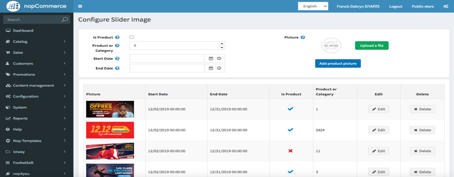
\includegraphics[width=16cm]{gestion_slider.png}
	\caption{Page de gestion des sliders.}
	\label{fig:sp0}
\end{figure}

Lorsque nous créons les sliders, l'utilsateur final peut voir ceci :

\begin{figure}[H]
	\centering
	
\includegraphics[width=8cm]{rendu_slider.png}
	\caption{Rendu des sliders sur l'application mobile.}
	\label{fig:sp0}
\end{figure}

\subsection{Page de gestion des push notifications.}

Dans cette page il s’agit de montrer comment on crée les push notifications, on modifie et on le supprime.

\begin{figure}[H]
	\centering
	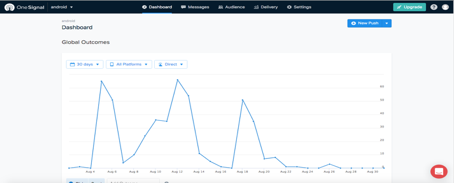
\includegraphics[width=16cm]{bord_onesignal.png}
	\caption{Tableau de bord onesignal.}
	\label{fig:sp0}
\end{figure}

La figure ci-dessus représente la liste des push notifications envoyées.

\begin{figure}[H]
	\centering
	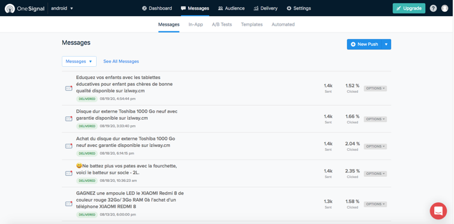
\includegraphics[width=16cm]{liste_push.png}
	\caption{Liste des push notifications.}
	\label{fig:sp0}
\end{figure}

\underline{Création d'un push notification}

La création d’un nouveau push notification est assez simple, il suffit pour cela de cliquer sur le bouton « New Push » du menu droit, ensuite la page de création s’affiche comme l’image qui suit.

\begin{figure}[H]
	\centering
	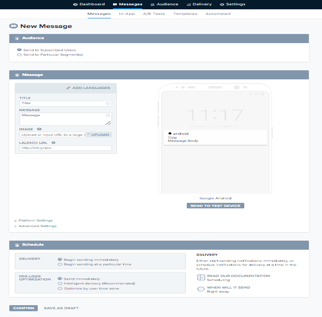
\includegraphics[width=16cm]{creation_push.png}
	\caption{Création d'un push notification.}
	\label{fig:sp0}
\end{figure}

Après l’envoi du push, on peut avoir ces statistiques liés 
\begin{figure}[H]
	\centering
	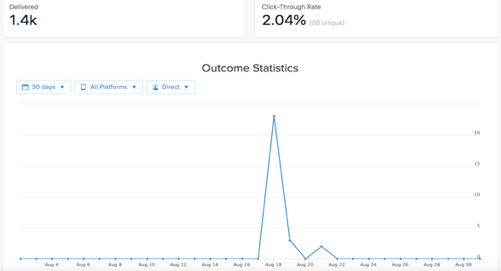
\includegraphics[width=16cm]{stat_onesignal.png}
	\caption{Statistiques d'envoi d'un message.}
	\label{fig:sp0}
\end{figure}

Lorsqu’on envoie un push notification voilà comment il se présente sur l’application
\begin{figure}[H]
	\centering
	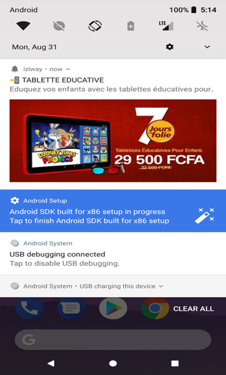
\includegraphics[width=8cm]{exple_push.png}
	\caption{Exemple d'un push notification reçu.}
	\label{fig:sp0}
\end{figure}

\subsection{Page de gestion des bloc catégorie et bloc produit .}

Dans cette page on renseigne les blocs catégories que nous voulons mettre en avant sur notre application et une fois les catégories mise en place nous allons pouvoir mettre en place les blocs produits correspondant aux différentes catégories.

\begin{figure}[H]
	\centering
	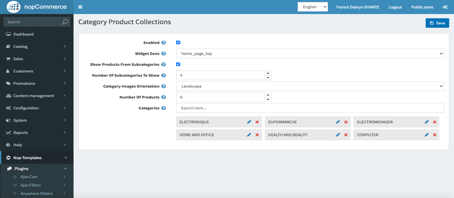
\includegraphics[width=16cm]{bord_categori}
	\caption{Tableau de bord de gestion de bloc categorie.}
	\label{fig:sp0}
\end{figure}

\begin{figure}[H]
	\centering
	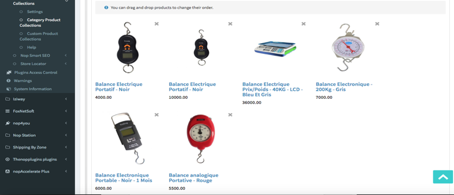
\includegraphics[width=16cm]{liste_produit.png}
	\caption{Liste des produits d'une catégorie (Bloc Produit).}
	\label{fig:sp0}
\end{figure}

\begin{figure}[H]
	\centering
	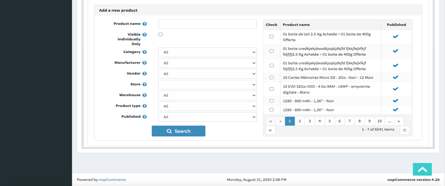
\includegraphics[width=16cm]{ajout_produit.png}
	\caption{Formulaire d'ajout des produits dans un bloc produit.}
	\label{fig:sp0}
\end{figure}

\subsection{Coût de mise en oeuvre de la solution .}

\begin{table}[H]
	\caption{Etude financière du matériel.}
	\label{Etude financière du matériel.}
	\centering
	\begin{tabularx}{\linewidth}{|X|X|X|}
		\hline \rowcolor{lightgray}  
		\textbf{Nom du produit} & \textbf{Caractéristiques} & \textbf{Total}\\
		\hline
		Serveur & Microsoft Azure offre Paas (Platform as Service) 3,20GHz, Disque Dur 250Go SSD, 3,5Go à 7Go de RAM & 500 000 FCFA \\
		\hline
		Ordinateur & MacBook Pro Intel Core i7 
Processor (2.2Ghz) 16Go / 255Go
Disque SSD, MacOS High Sierra
 &  250 000 FCFA \\
		\hline
		Google play console & Play Console  & 14 000 FCFA\\
		\hline
		\textbf{TOTAL}  &   &  \textbf{764 000 FCFA}  \\	
		\hline
	\end{tabularx}
\end{table}

Les utilisateurs de l’application devront être formés.

\begin{table}[H]
	\caption{Etude financière de la formation.}
	\label{Etude financière de la formation.}
	\centering
	\begin{tabularx}{\linewidth}{|X|X|X|X|}
		\hline \rowcolor{lightgray}  
		 \textbf{Prix de l'horaire} & \textbf{Nombres d'heures par utilisateur} & \textbf{Nombre d'utilisateurs} & \textbf{Montant} \\
		\hline
		 0 & 10 & 4 & 0 FCFA\\
		\hline
	\end{tabularx}
\end{table}

\begin{table}[H]
	\caption{Total coût de mise en oeuvre.}
	\label{Total coût de mise en oeuvre.}
	\centering
	\begin{tabularx}{\linewidth}{X|X|}
		\hline \rowcolor{lightgray}  
		 \textbf{ } & \textbf{Prix}\\
		\hline
		 Matériels & 764 000 FCFA \\
		\hline
		 Formation
 &  0 FCFA \\
		\hline
		 Coût de réalisation  & 8 320 000 FCFA\\
		\hline
		 TOTAL   &  \textbf{9 084 000 FCFA}  \\	
		\hline
	\end{tabularx}
\end{table}

\section{Discussion de la solution et bilan.}

La discussion de la solution est un point primordial, car elle permet de mesurer l’écart entre les prévisions et la réalisation. La mesure des écarts entre prévisions et réalisations, permettra d’apporter les correctifs nécessaires. 

Ainsi la structure de l’application a été évaluée en fonction des objectifs et exigences du cahier des charges, pour déterminer si le produit fini est conforme aux besoins exprimés. Cette évaluation a porté sur les aspects techniques et organisationnels du projet. Une autre sera organisée après le lancement officiel de l’application et sera axée sur son usage réel. 

\subsection{Evalutation technique .}

Dans un premier temps nous avons testé toutes les pages et liens pour s’assurer de leur bon fonctionnement. Étant donné qu’il y a un grand nombre de téléphones et que des problèmes de compatibilité peuvent se poser nous avons tesé l'application sur plusieurs téléphones, ensuite nous avons testé sa vitesse de téléchargement avant de faire des tests utilisateurs. 

\textbf{\underline{Tests sur téléphones}}

Nous avons déployé l’application iziway sur Google Play console. Le résultat s’est avéré très concluant, car nous n’avons pas remarqué une incompatibilité particulière avec les téléphones de différentes tailles.

\textbf{\underline{Tests utilisateurs}}

Le test utilisateur est une étape indispensable pour savoir si l’application a répondu aux besoins et attentes des utilisateurs. La facilité d’utilisation d’une application est un critère de satisfaction des visiteurs, aussi cette expérience est importante pour pouvoir rectifier les erreurs.

Ainsi nous avons testé avec comme utilisateurs le responsable marketing, le CEO de iziway, le responsable informatique et le responsable content-writer. Ces derniers ont été mis dans des conditions réelles permettant de réaliser de véritables opérations durant les tests. Nous avons fait en sorte qu’ils se sentent en confiance et que ce n’est pas eux qui sont testé, mais l’application.

De ce fait nous avons été neutres, sans jamais intervenir durant leurs passages sur l’application. Ces tests ont été assez positifs du fait de la simplicité de l’application tant du point de vue de la charte graphique que de l’arborescence. Certes il a fallu expliquer d’une fois comment les choses fonctionnent, car la première visite est toujours difficile du fait de la nouveauté à laquelle on  fait face. Il ressort de ces tests qu’il n’est pas difficile de se familiariser avec l’application.


\subsection{Respect du cahier des charges.}

Cette étape a nécessité la vérification du cahier des charges pour savoir si les différents points de ce dernier ont été bien réalisés. Aussi nous allons établir d’abord la méthodologie, ensuite nous allons procéder à l’évaluation proprement dite avant de faire une conclusion sur le résultats obtenus.

\textbf{\underline{Méthodologie}}

\begin{table}[H]
	\caption{Méthodologie.}
	\label{Méthodologie.}
	\centering
	\begin{tabularx}{\linewidth}{|X|X|X|}
		\hline \rowcolor{lightgray}  
		\textbf{Type d'indicateurs} & \textbf{Objet de vérification} & \textbf{Méthodologie}\\
		\hline
		Conformité & Le contenu et les fonctionnalités sont conformes aux points définis dans le cahier des charges  &Comparer le contenu et les fonctionnalités de l’application par rapport aux charges  \\
		\hline
		Efficience & Respect du temps de réalisation demandé
 &  Vérifier que tout a été réalisé dans le délai imparti \\
		\hline
		Performance & Temps de téléchargement, comptabilité avec les navigateurs  & Vérifier erreurs techniques et mauvais paramétrages\\
		\hline
	\end{tabularx}
\end{table}

\textbf{\underline{Evaluation}}

\begin{table}[H]
	\caption{Evaluation.}
	\label{Evaluation.}
	\centering
	\begin{tabularx}{\linewidth}{|X|X|X|}
		\hline \rowcolor{lightgray}  
		\textbf{Prévisions / cahier des charges} & \textbf{Réalisation} & \textbf{Résultats}\\
		\hline
		Gestion des blocs produits & Réalisé  & OK \\
		\hline
		Gestion des sliders & Réalisé & OK \\
		\hline
		Gestion des push notifications & Réalisé  & OK \\
		\hline
		Gestion des doubles bannières & Réalisé  & OK \\
		\hline
		Gestion des pop-ups & Réalisé  & OK \\
		\hline
	\end{tabularx}
\end{table}

\textbf{\underline{Évaluation de l’usage en temps réel de l’application}}

Cette évaluation de l’usage réel du portail est extrêmement importante, et sera effectué après le chargement des documents dans l’application et sa mise en service officielle. La question de l’usage revêt une importance particulière. Il est donc nécessaire d’évaluer l’impact des différentes mesures prises en la matière et l’intérêt du contenu de l’application au regard de l’utilisation réelle de celui-ci. 

Il s’agit en fait d’analyser ce que l’on appelle l’appropriation de la technologie par les utilisateurs, c’est-à-dire la manière dont ceux-ci adoptent la technologie. Par rapport à l’application, cela implique notamment d’évaluer quelles parties du site sont plus ou moins visitées par les utilisateurs, quels sont les fonctionnalités et services les plus utilisés. 

En définitive il s’agit de déterminer si l’application a rempli les objectifs de départs. En d’autres termes qu’est que le portail a apporté réellement à IZIWAY. Et tout ça en prenant en compte les commentaires spontanés fournis par les utilisateurs de l’application. 

Nous pouvons donc ressortir les différentes clés de performances sur l’application

\textbf{\underline{Concernant les nombres d'utilisateurs :}}

Étant donné que l’application été déployé en 20 décembre 2019 nos statistiques vont aller du 20 décembre 2019 au 31 août 2020 (date de fin de mon stage).

\begin{figure}[H]
	\centering
	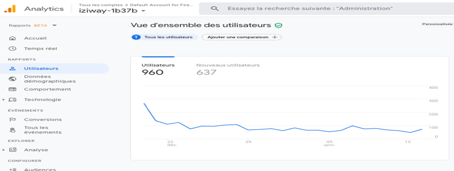
\includegraphics[width=16cm]{avant.png}
	\caption{Nombre d'utilisateurs avant le début du stage.}
	\label{fig:sp0}
\end{figure}

\begin{figure}[H]
	\centering
	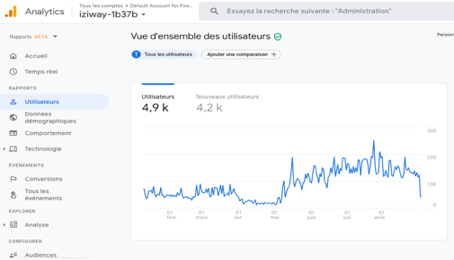
\includegraphics[width=16cm]{apres.png}
	\caption{Nombre d'utilisateurs après mon arrivé.}
	\label{fig:sp0}
\end{figure}

\textbf{\underline{Concernant les nombres de conversion :}}

\begin{figure}[H]
	\centering
	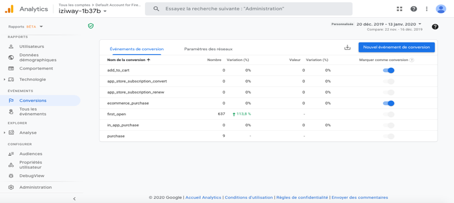
\includegraphics[width=16cm]{kpi_avant.png}
	\caption{Nombre de conversion avant mon arrivé.}
	\label{fig:sp0}
\end{figure}

\begin{figure}[H]
	\centering
	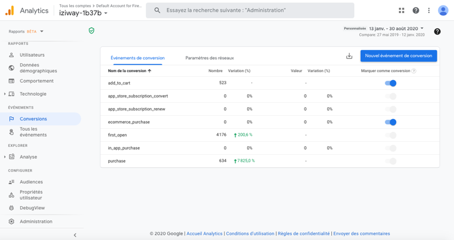
\includegraphics[width=16cm]{kpi_apres.png}
	\caption{Nombre de conversion après mon arrivé.}
	\label{fig:sp0}
\end{figure}

\subsection{Bilan.}

\textbf{\underline{Technique}}

Après 8 mois de travail, nous avons finalement terminé la plus grande partie du projet, et ne reste que le paramétrage. Ayant comme base de travail la mission assignée et le cahier des charges, nous avons optimiser l’application Android de la Marketplace IZIWAY CAMEROUN. Cette application étant un cadre de référence souple, est une porte d’entrée vers des contenus, des outils, qui permettent aux utilisateurs d’acheter et consulter.

De ce fait, il est amené à être évolutif donc en perpétuelle amélioration afin de mieux s’adapter aux besoins des utilisateurs. Ainsi une évaluation permanente sera effectuée pour mesurer les insuffisances de l’application et les nouveaux besoins. Dans cet ordre d’idées, d’autres services plus pointus pourraient être développés et ajoutés à l’application.

\textbf{\underline{Humain}}

Ce projet nous a permis de découvrir le cadre de travail, l’organisation, le personnel, bref la vie d’une entreprise. D’abord il y’a un cadre convivial avec des relations très fraternelles, et chaleureuses. Simplicité dans les relations car on ne sent pas les rapports hiérarchiques. Ensuite un esprit de groupe très développé, pour ne pas dire de travail d’équipe, on collabore et s’entraide pour atteindre les objectifs, même s’il y a des fois une certaine tendance au laxisme.

Avec des moyens modestes IZIWAY fait un travail extrêmement important pour la promotion et le développement du pays. Aussi nous avons été honoré de pouvoir apporter une modeste contribution par la réalisation de cette application qui, nous espérons, leur donnera des opportunités pour être soutenu dans leur action.


















































